\chapter{Research}
\label{cha:res}
This chapter provides a high level introduction to the concepts required to understand the functionality of Testu01. It also provides a guide to the control flow of the parts of the suite that have been parallelised. 
Furthermore, it examines previous attempts at creating parallel versions of Testu01. It explains the shortcomings of these attempts and the novelty in this implementation of a parallel Testu01.

\section{Current state of Testu01}
Testu01 is a C library that provides collections of tests, called test suites or batteries, for testing Random Number Generators. It provides a very extensive collection of tests that can be used to ensure that Random Number Generators adhere to adequate standards of quality. The tests allow "statistical testing of uniform random number generators"\cite{testu01-homepage}.

Apart from the tests, Testu01 is distributed with example programs that use batteries to test generators, as well as reference generators that are followed by warnings against using them in critical applications. Combined with a very thorough documentation, it is a very user friendly library and can be set up and used quickly by beginners.

The documentation is a particularly strong asset of Testu01. The Short and Full Guide pdf files are generated automatically from .tex sources during the build process. These same .tex sources are also used to generate the header files for the C code. As a result, the documentation is tightly integrated with the source code. It can be used both as conventional documentation that provides guidance in using Testu01 and as a guide to understanding the control flow of the source code and extending its functionality.

Testu01 also specifies very clear interfaces for generators. Files and generators implemented in software can be used as long as they adhere to the Testu01 specifications.

Despite its usability and extensive collection of tests, Testu01 suffers from performance issues. It was not designed to take advantage of multi-core processors. A singular instance of a generator can exist at each time and it cannot be shared between tests that run concurrently. The consequence of this is that if a battery is run on an idle multi-core system, one of the cores will be constantly at maximal capacity while the rest remain idle or are used exclusively for other processes.

\begin{figure}[h]
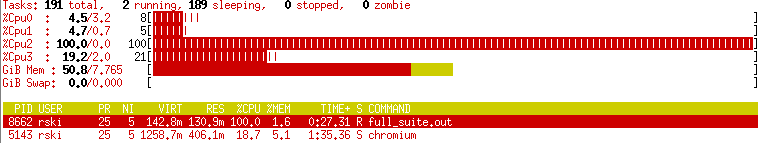
\includegraphics[scale=0.5]{top_full_suite}
\caption{Top displaying CPU usage while a test suite from Vanilla Testu01 is running\cite{full-suite}}
\label{fig:cpu_serial_tests}
\end{figure}

It is obvious that there is a large amount of computing capacity that is currently unused by Testu01. This is a serious problem that has been raised in the passed as an issue\cite{statistical-testing}. There have been attempts to address this, but they are either incomplete or have other issues which are discussed in more detail bellow.

\subsection{Control flow of Testu01}
The aim of the project is to parallelise the smallCrush, Crush and BigCrush batteries and so this section will provide a high level description of the typical control flow when one of these suites is used. The following are the essential components required for setting up and running one of these three batteries:
\begin{itemize}
  \item Executable: This file initialises the generator and calls the test suite. Written in C.
  \item bbattery\_\$SuiteName(): This is the function that calls the tests and collects their results. \$SuiteName can be SmallCrush, Crush or BigCrush.
  \item Generator: The tests use it to get the random numbers. Can be a file or a software based generator.
  \item Test functions: These are the functions that implement the statistical testing. The bbattery\_\$SuiteName() family of functions calls them.
  \item Result aggregators: The functions that are called at the end of the batteries. They collect the tests with suspect p values and print a list of the ones that the generator failed.
\end{itemize}

The following diagram shows the relationships between these components:

\subsection{Generators}
Testu01 provides an interface for linking and using external generators written in C.
There are three functions that have to be used to link an external generator with Testu01:
\begin{verbatim}
unif01_Gen *unif01_CreateExternGen01 (char *name, double (*gen01)(void));
unif01_Gen *unif01_CreateExternGenBits (char *name, unsigned int (*genB)(void));
unif01_Gen *unif01_CreateExternGenBitsL (char *name, unsigned long (*genB)(void));
\end{verbatim}

The Testu01 Guide provides a very detailed explanation on their use, along with examples. It is generally not good practice to duplicate documentation, and since external generators are not used in this project, please refer to the Testu01 on how to use them.

The generator that was used in this project is one of the uniform linear congruential generators (ULGCs) that was provided with Testu01.
From the Testu01 documentation\cite{testu01guide-p25}:
\begin{verbatim}
unif01_Gen * ulcg_CreateLCG (long m, long a, long c, long s);
\end{verbatim}

``Initializes a LCG of the form (2.1).
The initial state is x\textsubscript{0}= s and the output at step i is x\textsubscript{i}/m.
The actual implementation depends on the values of (m, a, c). Restrictions: a, c and s must be
non-negative and less than m.''

It is essentially a state machine. The state s determines the next "random" number and the initial state fully determines the sequence of numbers. When using a generator, states absolutely cannot be skipped. The generator has to move sequentially between them, otherwise the sequence is not valid.

Therein lies the problem with parallelising Testu01. Only one test can use the generator at a time or it will produce invalid sequences. For a parallel battery, each test needs to have a separate generator, with its own state, that is completely independent of the other tests' generators. By design, Testu01 uses only one generator per battery. This is the problem that every attempt to parallelise Testu01 has to solve.

\subsection{Batteries}
There are three test batteries in Testu01: \texttt{bbattery\_SmallCrush()}, \texttt{bbattery\_Crush(}) and \texttt{bbattery\_BigCrush()}.

\section{Previous Solutions}
\subsection{Parallel Implementation of the Testu01 Statistical Test Suite}
This is one of the oldest parallel Testu01 implementations. Suciu et al. parallelised two of the test suites using OpenMP and demonstrated a relatively high increase in performance for them. Although the profiling results are promising, this solution is quite limited. The reasons for that are explained bellow.

The suites that were parallelised are \textit{Alphabit} and \textit{Rabbit}. According to the Testu01 Long Guide\cite{longguide-alphabit}, these are batteries written to test hardware generators and can be run both on files and software based generators.

Suciu et al. achieved parallelism by using threads on top of the OpenMP parallel programming API\cite{openmp}. This allowed for fine grained control over which parts of the processing where shared between threads. Sharing the generators between threads, which is the biggest hurdle in parallelising Testu01, was overcome by copying the generators at the start of every thread. 

Using this approach, the first implementation of the Rabbit and Alphabit batteries was designed and implemented, ParTestU01. Although it did provide performance gains, the first test of Rabbit was significantly slower than the rest, as it accounted for roughly half of the execution time of the battery. This prevented ParTestU01 from scaling properly, as it was always limited to the execution time of the first test.

Thus, ParTestU01E was implemented. This takes advantage of the OpenMP capabilities in order to split the first test of Rabbit into more than one processes. This provided even more performance gains.

Ultimately, the speed up increase peaked between 5 and 9 threads. Increasing the thread number beyond nine was actually detrimental to the battery performance. Running parallel Rabbit on a 32MB and a 64MB file achieved an up to six times performance increase.

It would seem that these improvements brought to the test suite are quite significant. Unfortunately, they are not, especially compared to other suites. According to the Testu01 Guide, the file based Alphabit suite running on a 1.7Ghz processor takes 2.3 minutes to test a 2\textsuperscript{30} bit file. Similarly, Rabbit requires 28 minutes to test a file of the same size. Compared to running BigCrush with a simple generator, whose runtime is above three and a half hours on a much more modern processor, these times pale in comparison.

Furthermore, neither source code or binaries for this implementation seem to be available online. The paper provides an overview of the process of parallelising Testu01, but the project apparently is unpublished for wide distribution or extremely had to discover.

Finally the authors mention that they had started working on a new and improved parallel implementation at the time that this paper was published.

\subsection{Parallel Object-Oriented Implementation of the Testu01 Statistical Test Suites}
This is the paper that follows the previous one by Suciu et al. The same research group parallelised a different part of Testu01 using an Object Oriented approach. This is a very promising implementation with impressive performance gains compared to the original Testu01.

Once again, only part of Testu01 was parallelised. This was the Multinomial distribution test, as according to the authors this "is by far the most time consuming statistical test from Testu01". This solution is quite complex and was decided due to limitations of C, which could be overcome by features of OOP.

Generators for this solution were implemented using interfaces. In contrast with the original generator definitions, this allows for concurrent generators.The fact that generator data is now encapsulated along with functions for copying and initialising generators, allowed for concurrent generators.

Since C does not support object oriented programming, this solution was implemented in C\#. Similarly, OpenMP that was previously used had to be replaced with the Task Parallel Library (TPL).

Using these as a basis, the Multinomial Distribution Test was parallelised and performance metrics were gathered. The speedup is quite close but consistently higher than the one of the OpenMP implementation of this test.

The greatest advantage of this implementation is that it can be used to parallelise the rest of the tests of Testu01. Unfortunately, no paper on the progress of porting Testu01 to this TPL solution could be found.

\section{The Case for yet Another Solution}
\subsection{Problems with the current solutions}
Perhaps the biggest limitation of the previous solutions is their non-completeness. Testu01 is a very extensive library and provides a great number of batteries, tests and generators. These solutions improve a small fraction of them. There are still test suites that have runtimes of hours and could benefit greatly from multi-core scaling.

There is also still demand for a parallelised Testu01 that requires small changes in projects that already using Testu01. An implementation that uses the current  Testu01 specifications will have lower use barriers for projects that have conformed to them.

Furthermore, converting the entirety of Testu01 using these solutions is a time consuming and difficult challenge. The OpenMP solution turned out to not be usable outside of the Alphabit and Rabbit batteries, so it is not possible to use it as a guide for parallelising the rest of Testu01. Similarly, moving to TPL and C\# requires a considerable amount of effort. This project provides a solution that could be used to quickly parallelise any test suite and generator.

BigCrush is a test suite whose total run time exceeds three hours on a system with an Intel i5-3570k processor, with four cores clocked at 3.4Ghz. This suite calls 106 test functions, each one of which might run more than one test. Converting all these tests to a TPL based parallel suite and ensuring they still produce correct results is a task that might not be completed in the foreseeable future. This project will provide a parallel BigCrush that can be used with very minimal changes in existing programs that use Testu01 to test generators. The Crush and to a lesser extend smallCrush battery also benefit from it.
